\documentclass[a4paper]{jsarticle}
\usepackage[dvipdfmx]{graphicx}
\usepackage{amsmath}
\usepackage{bm}
\renewcommand{\thesection}{第\arabic{section}問}
\renewcommand{\thesubsection}{(\arabic{subsection})}
\renewcommand{\thesubsubsection}{(\alph{subsubsection})}
\begin{document}

\title{2013分野1}
\author{nakao}
\maketitle

\section{}
\subsection{}
つり合いを表す微分方程式は、
\begin{equation}
  E I w^{\prime \prime \prime \prime} = p
\end{equation}
と表せる。単純支持条件では梁の両端で鉛直方向の変位と曲げモーメントが0になるから、境界条件は
\begin{align}
  w(0) &= 0 \\
  w(L) &= 0 \\
  w^{\prime \prime}(0) &= 0 \\
  w^{\prime \prime}(L) &= 0
\end{align}
である。

\subsection{}
微小部分の力のつり合いより、曲げモーメントを$M(x)$とすると
\begin{equation}
  \frac{\mathrm{d}^2 M}{\mathrm{d} x^2} + p = 0
\end{equation}
が成り立つ。また、断面でのモーメントのつり合いから、
\begin{equation}
  M(x) = -E(x) I w^{\prime \prime}(x)
\end{equation}
が成り立つ。式(7)を式(6)に代入して、
\begin{equation}
  I \left(E(x) w^{\prime \prime \prime \prime}(x) + 
  2 E^{\prime}(x) w^{\prime \prime \prime}(x) + 
  E^{\prime \prime}(x) w^{\prime \prime}(x)\right)
  = p
\end{equation}
を得る。

\subsection{}
変化しない。
曲げモーメントは式(6)から求められ、この式はヤング率の分布によらない。

\subsection{}
増加する。
弾性変形のエネルギーは応力$\sigma$とひずみ$\varepsilon$を用いて
\begin{equation}
  \int \frac{1}{2} \sigma \varepsilon \mathrm{d} V
\end{equation}
で定義される。
ベルヌーイ・オイラーの仮定から
\begin{equation}
  \sigma = \frac{M}{I} z, \quad
  \varepsilon = \frac{M}{EI} z
\end{equation}
としてエネルギーを計算すると、
\begin{equation}
  \int \frac{1}{2} \sigma \varepsilon \mathrm{d} V
  = \int_0^L \int_A \frac{M^2}{2 E I^2} z^2 \mathrm{d} A \mathrm{d} x
  = \int_0^L \frac{M^2}{2 E I^2} \mathrm{d} x \int_A z^2 \mathrm{d} A
  = \int_0^L \frac{M^2}{2 E I} \mathrm{d} x
\end{equation}
を得る。$M,I$は損傷前後で変化せず、$E$のみが低下したとき、エネルギーは増加する。

\section{}
\subsection{}
$u_g = 0$のときのバネと重力のつり合い位置を$y = 0$として、
\begin{equation}
  m \ddot{y} + c \frac{\mathrm{d}}{\mathrm{d} t} \left(y - u_g(v t)\right)
  + k \left(y - u_g(v t)\right) = 0
\end{equation}
が成り立つ。

\subsection{}
$z = y - u_g(vt)$とすると、
\begin{equation}
  m \left(\ddot{z} + \frac{\mathrm{d}^2}{\mathrm{d} t^2} [u_g(vt)]\right)
  + c \dot{z} + k z = 0
\end{equation}
すなわち、
\begin{equation}
  m \ddot{z} + c \dot{z} + k z = m \omega^2 v^2 \sin (\omega v t)
\end{equation}
が成り立つ。この特解は、
$\phi = \arctan \frac{2 \xi \lambda}{1 - \lambda^2}$
を用いて
\begin{equation}
  z = \frac{m a \omega^2 v^2}{k}
  \frac{1}{\sqrt{(1 - \lambda^2)^2 + (2 \xi \lambda)^2}}
  \sin (\omega v t - \phi)
  = \frac{a \lambda^2}{\sqrt{(1 - \lambda^2)^2 + (2 \xi \lambda)^2}}
  \sin (\omega v t - \phi)
\end{equation}
と表せる。したがって、$y$の定常応答は、
\begin{equation}
  y = z + u_g(vt)
  = \frac{a \lambda^2}{\sqrt{(1 - \lambda^2)^2 + (2 \xi \lambda)^2}}
  \sin (\omega v t - \phi) + a \sin (\omega v t)
\end{equation}
となる。

\subsection{}
$R_d = 1/\sqrt{(1 - \lambda^2)^2 + (2 \xi \lambda)^2}$とする。
式(16)で$\sin (\omega v t - \phi)$を加法定理により展開することで
\begin{equation}
  y = (a \lambda^2 R_d \cos \phi + a) \sin (\omega v t)
  - a \lambda^2 R_d \sin \phi \cos (\omega v t)
\end{equation}
となるから、最大変位$y_m$は
\begin{equation}
  y_m = \sqrt{(a \lambda^2 R_d \cos \phi + a)^2
  + a \lambda^2 R_d \sin \phi \cos^2}
  = a \sqrt{\lambda^4 R_d^2 + 2 \lambda^2 R_d \cos \phi + 1}
\end{equation}
となる。ここで
\begin{equation}
  \cos \phi = \cos \left(\arctan \frac{2 \xi \lambda}{1 - \lambda^2}\right)
  = R_d (1 - \lambda^2)
\end{equation}
であることを用いると、
\begin{equation}
  y_m = a \sqrt{\lambda^2 (2 - \lambda^2) R_d^2 + 1}
\end{equation}
が得られる。よって、
\begin{equation}
  \eta = \frac{y_m}{a} = \sqrt{\lambda^2 (2 - \lambda^2) R_d^2 + 1}
\end{equation}
である。\par
$\xi = 0$のとき、$R_d = \frac{1}{|1 - \lambda^2|}$であるから、
\begin{equation}
  \eta = \frac{1}{|1 - \lambda^2|}
\end{equation}
となる。\par
$\xi = 1/3$のとき、$R_d = \frac{3}{\sqrt{9 \lambda^4 - 14 \lambda^2 + 9}}$であるから、
\begin{equation}
  \eta = \sqrt{\frac{4 \lambda^2 + 9}{9 \lambda^4 - 14 \lambda^2 + 9}}
\end{equation}
となる。式(22),(23)のグラフは図1の通り。\par
\begin{figure}[htb]
  \centering
  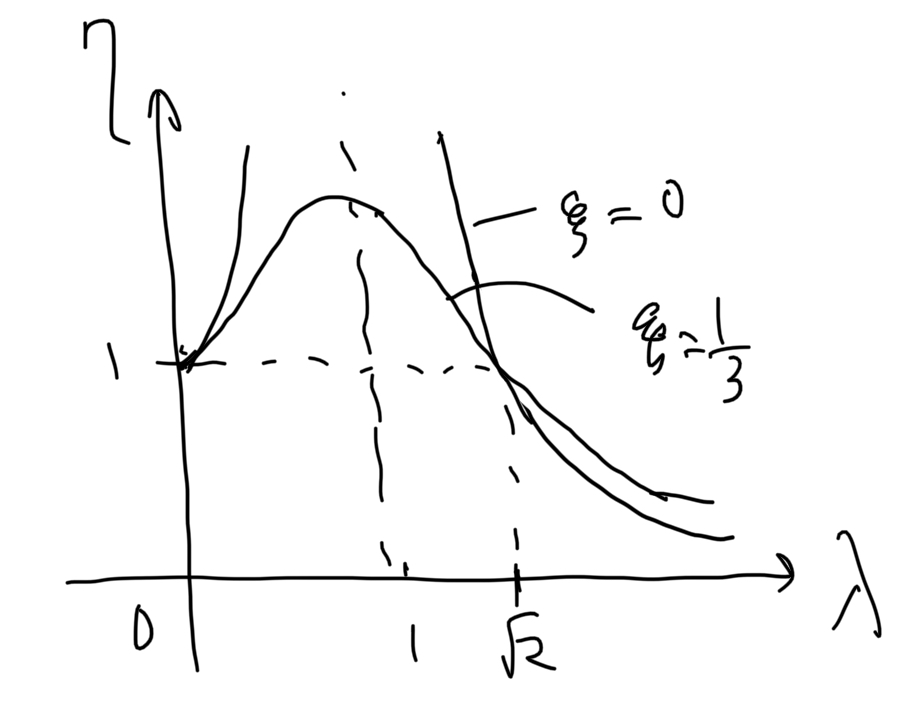
\includegraphics[width=0.3\hsize]{fig1.png}
\end{figure}
また、式(21)より$\eta$が$\xi$に依存しないためには、
\begin{equation}
  \lambda^2 (2 - \lambda^2) = 0
\end{equation}
であればよい。$\lambda \geq 0$の範囲でこれを満たすのは、
$\lambda = 0, \sqrt{2}$である。

\subsection{}
運動方程式は式(12)で$c = 0$として、
\begin{equation}
  m \ddot{y} + k y = k u_g(vt)
\end{equation}
と表せる。車両には
$k u_g (vt)$の外力が作用する。\par
$0 \leq t \leq \frac{d}{v}$の期間で車両に加わる力積は
\begin{equation}
  \int_0^{\frac{d}{v}} k u_g (vt) \mathrm{d} t
  = \int_0^{\frac{d}{v}} k b \sin \left(\frac{\pi v t}{d}\right) \mathrm{d} t
  = \frac{2 m \omega_0^2 b d}{\pi v}
\end{equation}
である。荷重を衝撃作用とみなせば、この期間の外力は
$\frac{2 m \omega_0^2 b d}{\pi v} \delta(t)$である。\par
同様に、
$\frac{d}{v} + \frac{\pi}{\omega_0} < t \leq \frac{2d}{v} + \frac{\pi}{\omega_0}$
の期間で車両に作用する外力は、
\begin{equation}
  \frac{2 m \omega_0^2 b d}{\pi v} \delta \left(t - \left(\frac{d}{v} + \frac{\pi}{\omega_0}\right)\right)
  = \frac{2 m \omega_0^2 b d}{\pi v} \delta \left(t - \frac{1}{\omega_0}\left(\frac{d \omega_0}{v} + \pi\right)\right)
  \simeq \frac{2 m \omega_0^2 b d}{\pi v} \delta \left(t - \frac{\pi}{\omega_0}\right)
\end{equation}
とみなせる。\par
したがって、解くべき運動方程式は、
\begin{equation}
  m \ddot{y} + k y =
  \frac{2 m \omega_0^2 b d}{\pi v} \left(\delta(t) +
  \delta \left(t - \frac{\pi}{\omega_0}\right)\right)
\end{equation}
となる。
解はDuhamel's Integralにより
\begin{equation}
  y = \frac{1}{m \omega_0}
  \int_0^t \sin \omega_0 (t - \tau) 
  \frac{2 m \omega_0^2 b d}{\pi v} \left(\delta(t) +
  \delta \left(t - \frac{\pi}{\omega_0}\right)\right) \mathrm{d} \tau
\end{equation}
で与えられる。\par
$0 < t < \frac{\pi}{\omega_0}$のとき、
\begin{equation}
  y = \frac{2 \omega_0 b d}{\pi v} \sin \omega_0 t
\end{equation}
となる。\par
$\frac{\pi}{\omega_0} \leq t < \frac{2\pi}{\omega_0}$のとき、
\begin{equation}
  y = \frac{2 \omega_0 b d}{\pi v}
  \left(\sin \omega_0 t + \sin \omega_0 \left(t - \frac{\pi}{\omega_0}\right)\right) =0
\end{equation}
となる。
したがって、
\begin{equation}
  y =
  \begin{cases}
    \frac{2 \omega_0 b d}{\pi v} \sin \omega_0 t & \left(0 < t < \frac{\pi}{\omega_0}\right)\\
    0 & \left(\frac{\pi}{\omega_0} \leq t < \frac{2\pi}{\omega_0}\right)
  \end{cases}
\end{equation}
である。
\end{document}